\section{The Gisele clinical pathway analyzer\label{section:tool-clinical-pathway-analyzer}}

A clinical pathway is a well-defined process, based on medical protocols, guidelines and recommendations; centered on a specific patient class with similar needs; involving a multi-disciplinary team; and addressing clear clinical goals \cite{Middleton:2000}. The tool presented in this section is motivated by a joint project aimed at building and analyzing models of clinical pathways. Guarded hMSCs have been chosen as the particular kind of process models, for which analyses discussed in \cite{Damas:2011} have been implemented.

A snapshot of the main screen of the tool is shown in Fig.~\ref{image:gisele-tool}. Interrested readers will find a guided tour on a medical case-study in \cite{Damas:2011}. In this section, we will highlight keypoints of its implementation and discuss a few design decisions. The main features implemented in the tool are:

\begin{figure}[H]
\centering\scalebox{.525}{
  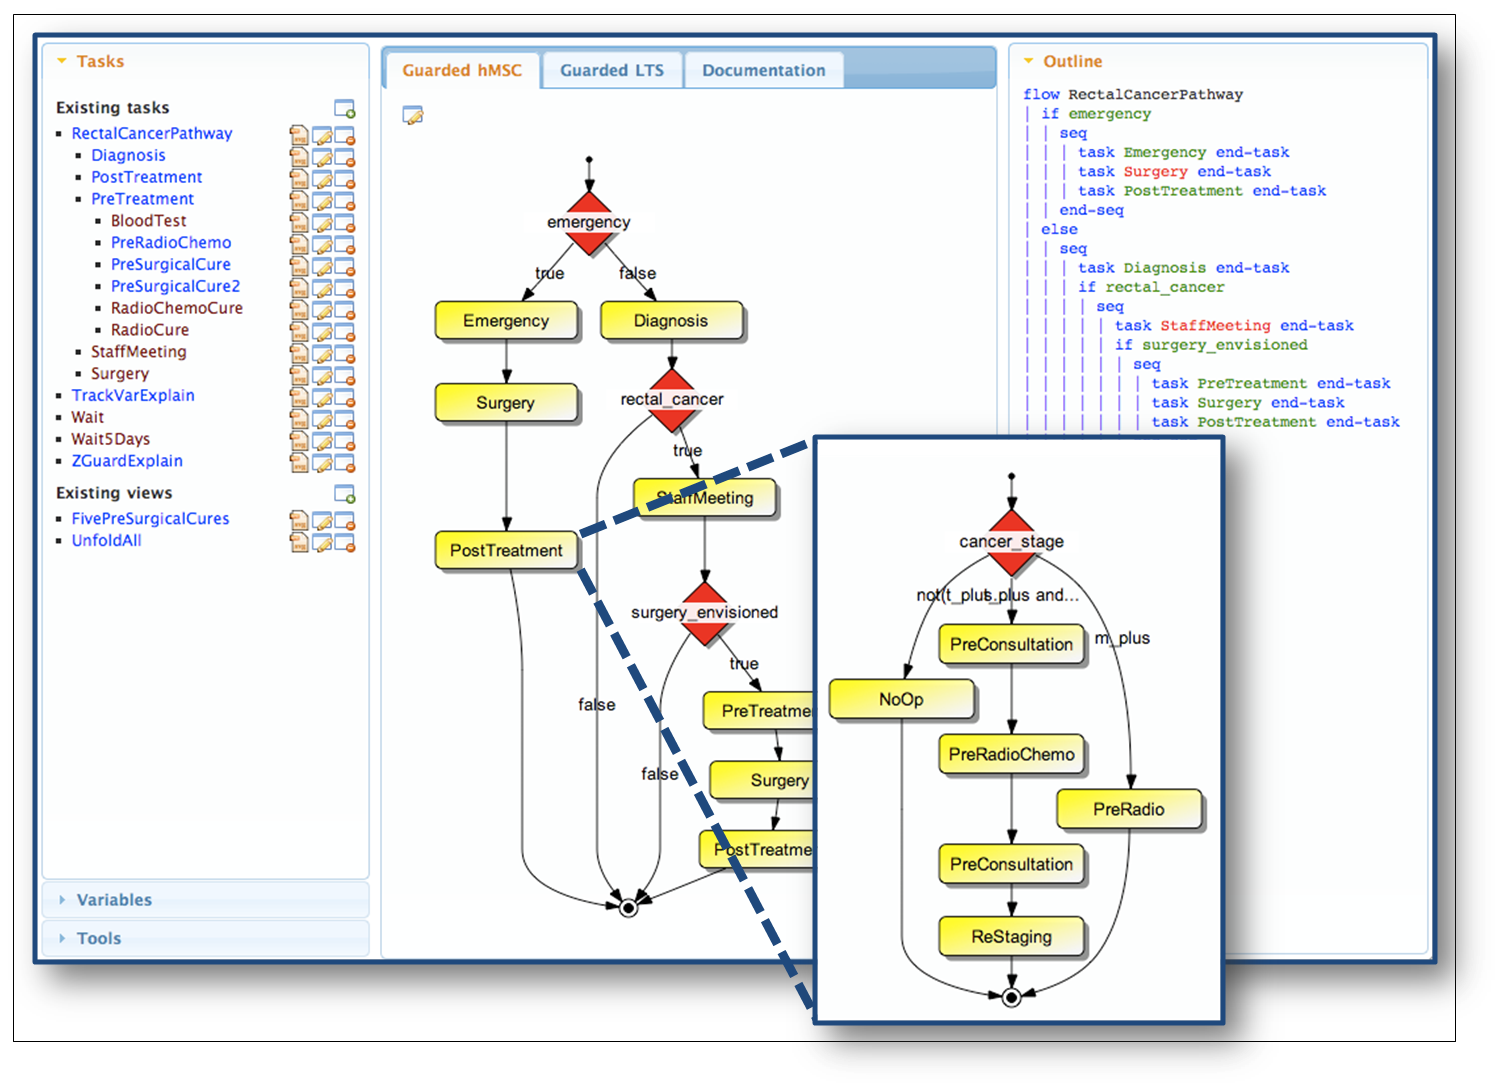
\includegraphics[trim=5mm 10mm 10mm 5mm, clip]{src/7-tool-support/images/gisele-tool}}
  \caption{The Gisele tool, a clinical pathway analyzer\label{image:gisele-tool}}
\end{figure}

\begin{itemize}
\item The modeling and visualization of process models made of tasks and decision nodes defined on fluents (see Section \ref{section:background-process-models}). Tasks can be successively refined in sub-processes, as illustrated in Fig.~\ref{image:gisele-tool}.
\item A variety of analyses for checking the completeness, non overlapping and accuracy of decision nodes; verifying pre-conditions of tasks; analyzing processes in terms of timing and dosage; and so on (see \cite{Damas:2011}).
\item Dedicated screens for eliciting process models; documenting them with stakeholders; unfolding process models for specific analyses; projecting them on specific patient classes, and so on.
\end{itemize}

\subsection*{Architecture and design decisions}

The architecture of the tool is illustrated in Fig.~\ref{image:gisele-tool-architecture}. Its main modules are explained below in the light of our main design decisions.

\begin{figure}[H]
\centering\scalebox{.5}{
  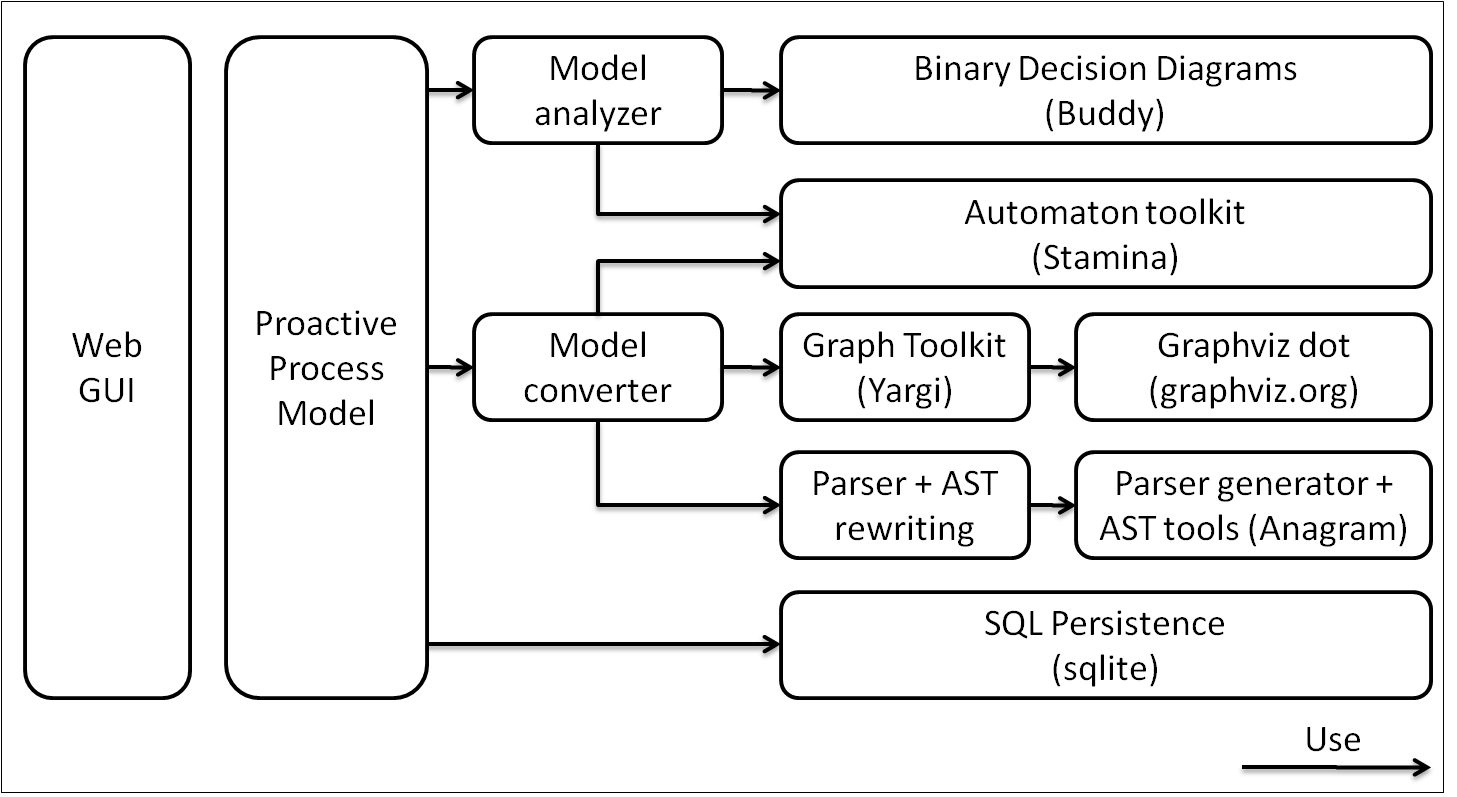
\includegraphics[trim=3mm 3mm 3mm 3mm, clip]{src/7-tool-support/images/gisele-tool-architecture}}
  \caption{Architecture of the Gisele tool\label{image:gisele-tool-architecture}}
\end{figure}

\begin{description}
\item[Process language] To keep the tool simple to use and to develop, a simple process language is used instead of a graphical process editor. This module defines a grammar and an API on top of parsing and abstract syntax tree rewriting tools from the \emph{anagram} library.

The process language uses common abstractions from structured programming, i.e. sequencing of tasks, if/then/else, guarded commands (case), while and until loops, and so on. For example, the meeting scheduling process could be encoded as follows:

\ldots

\item[Rich pathway model] A complete pathway model is composed of several tasks in successive refinements, fluent definitions, task documentation, and so on. This structural module implements a rich model for clinical pathways; they are also kept persistent with the use of a SQL database.

This module and its use of the ``Process rewriting'' and ``Process analyzer'' is an important design decision of the Gisele tool: doing the opposite of the ISIS tool with respect to analyses and user feedback. 

In the ISIS tool, synthesis and analyses is made ``on demand'': for example, the user explicitely launches consistency checks and receives dedicated feedback as a result (see Section \ref{section:tool-support-isis}).

The Gisele tool reverses this by considering a richer model with a strong support for views. This architectural pattern sees analysis results as part of the model itself, yet computed, instead of being external to the model. Among others, this facilitates the implementation of graphical interfaces and provides a rich and natural user experience. Indeed, analysis-related queries and views are made simple:

\begin{itemize}
\item list all decision nodes for which guards are incomplete;
\item highlights the structure of a process with tasks with the pre-condition violated in red;
\item \ldots
\end{itemize}

\item[Process rewriting] The implementation of the rich pathway model relies on specific algorithms for rewriting processes as multiple views. For example, a process instance is parsed and kept as an abstract syntax tree (AST); rewrited as a guarded hMSC for being displayed; compiled in an equivalent guarded LTS for analyses; and so on. 

Rewritings algorithms are implemented in the ``Process rewriting'' module, and rely on external libraries for parsing, rewriting ASTs, manipulating graphs and automata. This module also provides traceability support between the multiple views to the rich model.

\item[Process analyzer] This module implements the process analyses discussed in \cite{Damas:2011}, through multiple concretization of an abstract fix-point algorithm on guarded LTS. It makes intensive uses of automata and binary decision diagrams with the help of dedicated libraries. 

Results of all analyses are kept as decoration of g-LTS states. The rich model triggers analysis executions when such decorations are needed for answering queries and computing views. It also keep analysis results in cache to avoid making costly checks too often.

\item[Web GUI] The last module is the graphical user interface (GUI), that mostly runs inside a web browser. Thanks to services offered by the rich model, the implementation of the GUI turns to a simple model navigator, implemented internaly with an MVC pattern. 

The main screen of this navigator is made of three panels (see Fig~\ref{image:gisele-tool}). The left one gives a global outline of the clinical pathway and allows navigating between its different tasks. The current task is always displayed as a process graph in the middle panel, and as an annotated abstract syntax tree in the right panel. This tree also provides analysis feedback to the user: tasks and decision nodes for which at least one analysis fails are displayed in red; clicking on a node on this tree gives a detailed analysis explanation and counter-examples on analysis failures.

\end{description}


